\documentclass{beamer}

\usepackage{graphicx}
\usepackage{siunitx}
%for boxes
\usepackage{tcolorbox}
\usepackage{amsmath}
\usetheme{UoB}
\addtobeamertemplate{navigation symbols}{}{%
    \usebeamerfont{footline}%
    \usebeamercolor[fg]{footline}%
    \hspace{1em}%
    \insertframenumber/\inserttotalframenumber
}


\newcommand{\vc}[1]{\vec{\boldsymbol{#1}}}
\newcommand{\hr}{\hat{\boldsymbol{r}}}
\newcommand{\hi}{\hat{\boldsymbol{i}}}
\newcommand{\hj}{\hat{\boldsymbol{j}}}
\newcommand{\hk}{\hat{\boldsymbol{k}}}
\usepackage{mathtools}
\newcommand\deq{\stackrel{\mathclap{\tiny\mbox{def}}}{=}}
\usepackage{soul}

%block size
\setbeamerfont{block title}{size=\small}

\makeatletter
\let\HL\hl
\renewcommand\hl{%
  \let\set@color\beamerorig@set@color
  \let\reset@color\beamerorig@reset@color
  \HL}
\makeatother

\usefonttheme{serif}
%\usefonttheme{professionalfonts}
 \usepackage{eulerpx} % Euler math font
\usepackage{color} \definecolor{lightblue}{rgb}{.90,.95,1} 
\sethlcolor{lightblue}

\usepackage{animate}
\title[Short Title]{Potentials and Fields}
\subtitle{in the context of electromagnetism}
\author{Francesco Turci}
\institute{School of Physics}
\date{7th February 2023}


%solve eulerpx bug
\DeclareMathSymbol{\infty}{\mathord}{symbols}{49}
\begin{document}
\lecture{Lecture 1}{01}


\begin{frame}[leftcolor=white,rightcolor=UniversityRed,div=0.8\paperwidth]
  \titlepage
\end{frame}


%%%%%%%%%%%%%%%%%%%%

\begin{frame}
\frametitle{Repository \& references}
The slides and attached resources can be found at

{\color{UniversityRed}\href{https://github.com/FTurci/potential_and_fields}{https://github.com/FTurci/potential\_and\_fields}}\newline

Additional context and information can be found in
\begin{itemize}
	\item Chapter 23, \textit{Physics for Scientists and Engineers}, Tipler \& Mosca, 6th edition, 
(Freeman, 2007) 
\item Chapter 23, \textit{University Physics with Modern Physics}, 
Young \& Freedman, 15th edition, (Pearson, 2019) 
\end{itemize}
\end{frame}

%%%%%%%%%%%%%%%%%%%%
\begin{frame}
	\frametitle{Goals}
	\begin{itemize}
		\item Recall the ideas behind conservative forces and potential energy.
		\item Introduce the concept of potential in electrostatics.
		\item Contrast the electric and magnetic cases. 
	\end{itemize}
\end{frame}

%%%%%%%%%%%%%%%%%%%%
\begin{frame}

\frametitle{Conservative forces and path independence}
\footnotesize

%Under the action of conservative forces, the \textbf{mechanical energy is conserved}.
%\begin{equation}
%E^{i} = K^{i}+U^i = K^{f}+U^f= E^f.
%\end{equation}
%Hence
%\begin{equation}
%	\Delta U = U_f-U_i = - (K_f-K_i)
%\end{equation}
%
%\pause
%\textbf{Work} can be introduced via the kinetic energy theorem
%\begin{equation}
%	W  =K_f-K_i,
%\end{equation}
%so that (using the scalar product notation for W)

%\pause
%\hl{
The \textbf{work} $W$ done by a \textbf{conservative} force only depends on the \textbf{initial} and \textbf{final} positions. It defines the \textbf{potential energy difference} $\Delta U$:

\begin{block}{}
\begin{equation}
	\Delta U = U_f-U_i = - W   = -\int_i^f \vc{F}\cdot d\vc{\ell}
\end{equation}
\end{block}
\begin{center}
	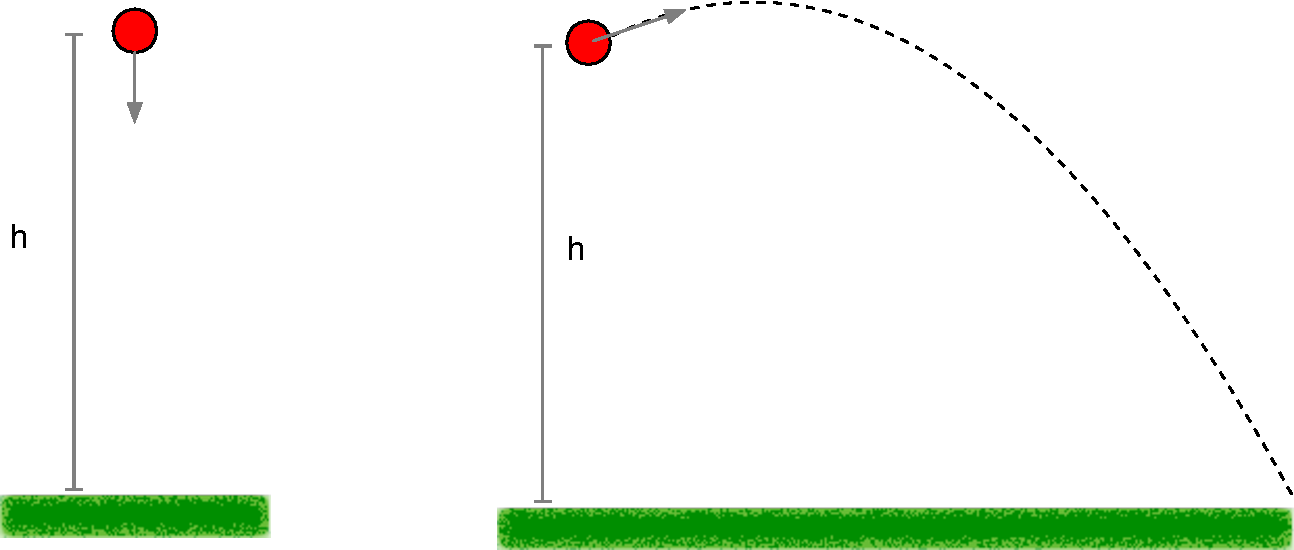
\includegraphics[width=0.7\columnwidth]{figs/paths}

\end{center}

\textbf{Example: gravity}
\begin{equation}
	\Delta U = m g h
\end{equation}
\textit{The potential difference does not depend on the paths taken by the particle but only on the initial and final heights. }
	
\end{frame}

%%%%%%%%%%%%%%%%%%%%
\begin{frame}
	\frametitle{Gravitational potential energy and potential}
%	\small
Gravity is \textbf{conservative}. For masses $m$ and $M$ at distance $\vc{r}$ the force and the potential energy are
\begin{block}{}
\begin{equation}
  \vc{F}_g(\vc{r}) =- G\dfrac{m M }{r^2}\hr  \end{equation}
 \begin{equation}
  U(r) = -G\dfrac{mM}{r}
\end{equation}
\end{block}

\begin{center}
	\includegraphics[width=0.3\textwidth ]{figs/gravity}
\end{center}
\end{frame}

%%%%%%%%%%%%%%%%%%%%
\begin{frame}
\frametitle{Gravitational potential energy and potential}
We can also define the \textbf{gravitational vector field} probed by a point particle $m$ at any $\vc{r}$
\begin{equation}
  \vc{g}(\vc{r}) = \dfrac{\vc{F}_g}{m}=- G\dfrac{M }{r^2}\hr 
\end{equation}\pause
Path independence means that for any path $\gamma(\vc{r}_1,\vc{r}_2)$ there exists a \textbf{scalar function} $\phi$ such that
\begin{block}{}
\begin{align}
   \phi(\vc{r}_2)-\phi(\vc{r}_1)&=\dfrac{U(\vc{r}_2)}{m}-\dfrac{U(\vc{r}_1)}{m}= -\int_{\gamma}\vc{g}\cdot d\vc{\ell}
\end{align}
\end{block}
It is the \textbf{gravitational potential} $\phi$.



%The potential energy to move  the masses from distance $\vc{r}_0$ to distance $\vc{r}$ is
%
%
%
%\begin{equation}
%  \Delta U =  -\int_{\vc{r}_0}^{\vc{r}}\vc{F}_g(\vc{r}') \cdot d\vc{r}'=-GmM\int_{r_0}^{r} r'^{-2}dr'= -G\dfrac{mM}{r}+G\dfrac{mM}{r_0}
%\end{equation}
\end{frame}


%%%%%%%%%%%%%%%%%%%%
\begin{frame}
	\frametitle{Path independence, scalar potential and gradient}
	\small
%	Take any path $\gamma(\vc{r}_1,\vc{r}_2)$.
%	Path independence 	
%\begin{equation}
%  \phi(\vc{r}_2)-\phi(\vc{r}_1)=-\int_{\gamma}\vc{g}\cdot d\vc{\ell}\end{equation}
In  one dimension, path independence is equivalent to
\begin{equation}
  \phi(x_2)-\phi(x_1)=-\int_{x_1}^{x_2}g(x)dx\rightarrow g(x) = -\dfrac{d\phi}{dx}
  \end{equation}
  
 In higher dimensions, it generalises to the \textbf{gradient theorem}: 
 
 \begin{equation}
    \phi(\vc{r}_2)-\phi(\vc{r}_1)=-\int_{\gamma}\vc{g}\cdot d\vc{\ell}\rightarrow g(\vc{r})=-\vc{\nabla}\phi(\vc{r})
\end{equation}

The \textbf{vector field} $\vc{g}$ is the \textbf{gradient of the potential}.
\begin{equation}
	\vc{\nabla}\phi(x,y,z) = \dfrac{\partial \phi}{\partial x}\hi+\dfrac{\partial \phi}{\partial y}\hj+\dfrac{\partial \phi}{\partial z}\hk
\end{equation}
\end{frame}





\begin{frame}
	\frametitle{Conservative fields}
	\footnotesize
\begin{columns}[T]
\begin{column}{0.5\textwidth}{
\setbeamercolor{block body}{bg=white}
\setbeamercolor{block title}{bg=white}
\begin{block}{Gravity}
%\textbf{Gravity}\newline
Force:
$$
 \vc{F}_g(\vc{r}) =- G\dfrac{Mm }{r^2}\hr
$$
Vector field:
$$
  \vc{g}(\vc{r}) =\dfrac{\vc{F}_g(\vc{r})}{m}=- G\dfrac{M }{r^2}\hr
$$
Potential (scalar field):
$$
\phi(\vc{r})=-G\dfrac{M}{r}
$$
Verify that 
$$\vc{g}=-\vc{\nabla}\phi$$
\end{block}}
\end{column}
\begin{column}{0.5\textwidth}\pause
\begin{block}{Electrostatics}
%\textbf{Electrostatics}
%\newline
Force:
\vspace{12pt}
$$
  \vc{F}_e(\vc{r}) =
\dfrac{k qQ}{r^2}\hr
$$
\pause
Vector field:
$$
  \vc{E}(\vc{r}) =\dfrac{ \vc{F}_e(\vc{r})}{q}=\dfrac{kQ }{r^2}\hr
$$
\pause
Potential (scalar field):
$$
V(\vc{r})=\dfrac{kQ}{r}
$$
Again
\vspace{7.5pt}
$$\vc{E} = -\vc{\nabla}V$$
\end{block}
\end{column}
	
\end{columns}


\end{frame}

\begin{frame}
	\frametitle{Electric potential}
	\small
	Two relationships between the electric field and potential
\begin{block}{}
\begin{align}V(\vc{r})-V_{0}&=-\int_{\gamma}\vc{E} \cdot d \vc{\ell}\\
\vc{E} &= -\vc{\nabla}V
\end{align}
\end{block}

	
	\begin{itemize}
%	\item $V(\vc{r})$ is a \textbf{scalar} function , $\mathbb{R}^3\rightarrow\mathbb{R}$
	\item Only $\Delta V$ is physically significant, i.e. one must define a reference configuration $\vc{r}_0$ with zero potential $V_0=0$. 
	\item The potential is measured in \textbf{Volt}, $\unit{1\volt}= 1\unit{\joule}/1\unit{\coulomb}$
	\item In directions \textbf{orthogonal} to the field, the potential does not vary $\rightarrow$ \textbf{equipotential contours}.
\end{itemize}
\end{frame}


%
%\begin{frame}
%
%\frametitle{Electric potential difference}
%\small 
%We can define the electrostatic field from the electrostatic force  using the test charge $q$:
%\begin{equation}
%	\vc{E}= \dfrac{\vc{F}_e}{q}
%\end{equation}
%For an infinitesimal displacement, the definition of $\Delta U$ (eq.\ref{eq:udef}) implies
%
%\begin{equation}
%	dU = - \vc{F}_e\cdot d\vc{\ell}= -q\vc{E}\cdot d\vc{\ell}.
%\end{equation}\pause
%This suggests defining a new quantity
%\begin{block}{Potential Difference}
%\begin{equation}
%	dV = -\vc{E}\cdot d\vc{\ell}.
%\end{equation}
%\end{block}
%and naturally $dU = q dV$.
%
%\end{frame}




%\begin{frame}
%\frametitle{The electric potential}
%\small
%
%Let us consider $dV = -\vc{E}\cdot d\vc{\ell}$ and different possible displacements $d\vc{\ell}$.
%
%\begin{itemize}
%	\item If $d\vc{\ell}\perp\vc{E}\rightarrow dV=0$.
%	\item If $d\vc{\ell}\parallel \vc{E}\rightarrow dV=dV_{\text{max}}$
%\end{itemize}
%The projection of $\vc{E}$ along the displacement is 
%
%\begin{equation} \vc{E}\cdot d\vc{\ell}= E cos\theta d\ell \deq E_t d\ell \rightarrow E_t = -\dfrac{dV}{d\ell}
%\end{equation}
%\pause
%Suppose we know $dV$ and want to retrieve $\vc{E}$. We now know that
%\begin{itemize}
%	\item we need to move by $d\vc{\ell}$ in the direction of greatest change in $V$
%	\item the magnitude of $\vc{E}$ in that direction is the derivative along $d\vc{\ell}$
%\end{itemize}
%These are the defining properties of the \textbf{gradient} of $V$.
%
%
%
%\end{frame}

%\begin{frame}
%\frametitle{Electric potential}
%\small
%
%%
%%The potential difference 
%%
%%\begin{equation}\Delta V = \int_i^f dV = V_f-V_i =-\int_i^{f}\vc{E}\cdot d\vc{\ell}\end{equation}. 
%%
%%This signifies that the integral over the path connecting $i$ and $f$ only on the
%%
%% we link the vector field $\vc{E}$ to the potential 
%
%\begin{block}{Field as gradient of potential}
%\begin{equation}
%		-{\rm grad} V(\vc{r}) = -\vc{\nabla}V(\vc{r}) = \vc{E}(\vc{r})
%\end{equation}
%\end{block}
%Naturally \begin{equation}\Delta V = V(\vc{r})-V(\vc{r}_0) =\int_{\gamma(\vc{r}_0, \vc{r})} \vc{\nabla}V(\vc{r})d\vc{r}=-\int_{\gamma(\vc{r}_0, \vc{r})} \vc{E}(\vc{r})d\vc{r},
%\end{equation}
%on any path $\gamma$ between $\vc{r}_0$ and $\vc{r}$.
%\pause
%\begin{itemize}
%%	\item $V(\vc{r})$ can be evaluated along any path, and takes value for any point in space $\vc{r}$.
%	\item $V(\vc{r})$ is a \textbf{scalar} function , $\mathbb{R}^3\rightarrow\mathbb{R}$
%	\item Only $\Delta V$ are physically significant, i.e. one must define a reference configuration $\vc{r}_0$ with zero potential $V=0$. 
%	\item The potential is measured in \textbf{Volt}, $\unit{1\volt}= 1\unit{\joule}/1\unit{\coulomb}$
%\end{itemize}
%
%\end{frame}





\begin{frame}
\frametitle{Coulomb potential}
\small

Consider the field emanating from a charge $q$. Taking the integral definition of $V$ and a reference point at $r_{0}=+\infty$ with $V(\infty)=0$ we have
\begin{align}V(\vc{r})-V_{\infty }&=-\int_{\infty }^{\vc{r}} 
\vc{E} \cdot d \vc{\ell}=-\int_{\infty }^{\vc{r}}
\frac{k q}{r'^2} \hat{r'} \cdot d \vc{\ell}\\
&=-
\int_{\infty }^{r} \frac{k q}{r'^2} d r'= -kq\left(-r^{-1}-0\right)\\
&=\dfrac{kq}{r}
\end{align}
\pause
%\begin{block}{Coulomb potential}
	\begin{equation}
		V(r) = \dfrac{kq}{r} \quad \text{(central potential)}
	\end{equation}
\end{frame}


% animation
\begin{frame}
\frametitle{Coulomb potential}
\begin{center}
	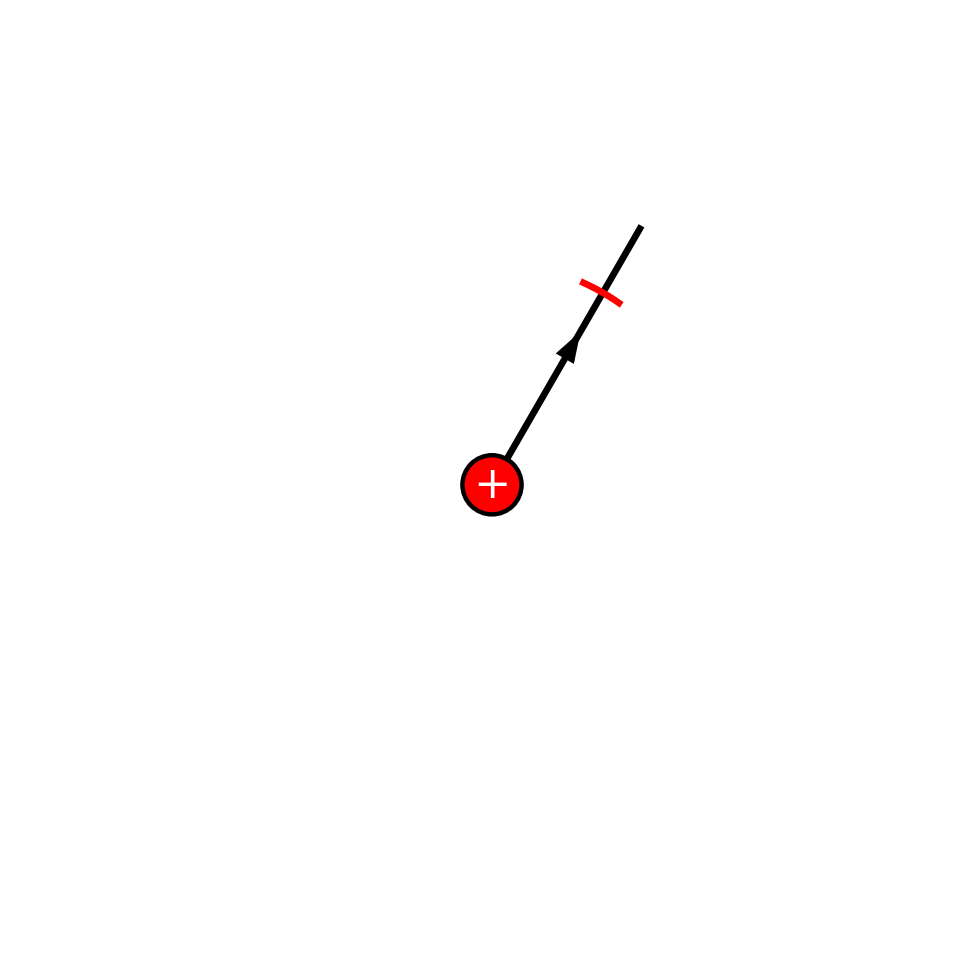
\includegraphics[width=0.75\columnwidth]{figs/seq/frame1}
\end{center}
\end{frame}
\begin{frame}
\frametitle{Coulomb potential}
\begin{center}
	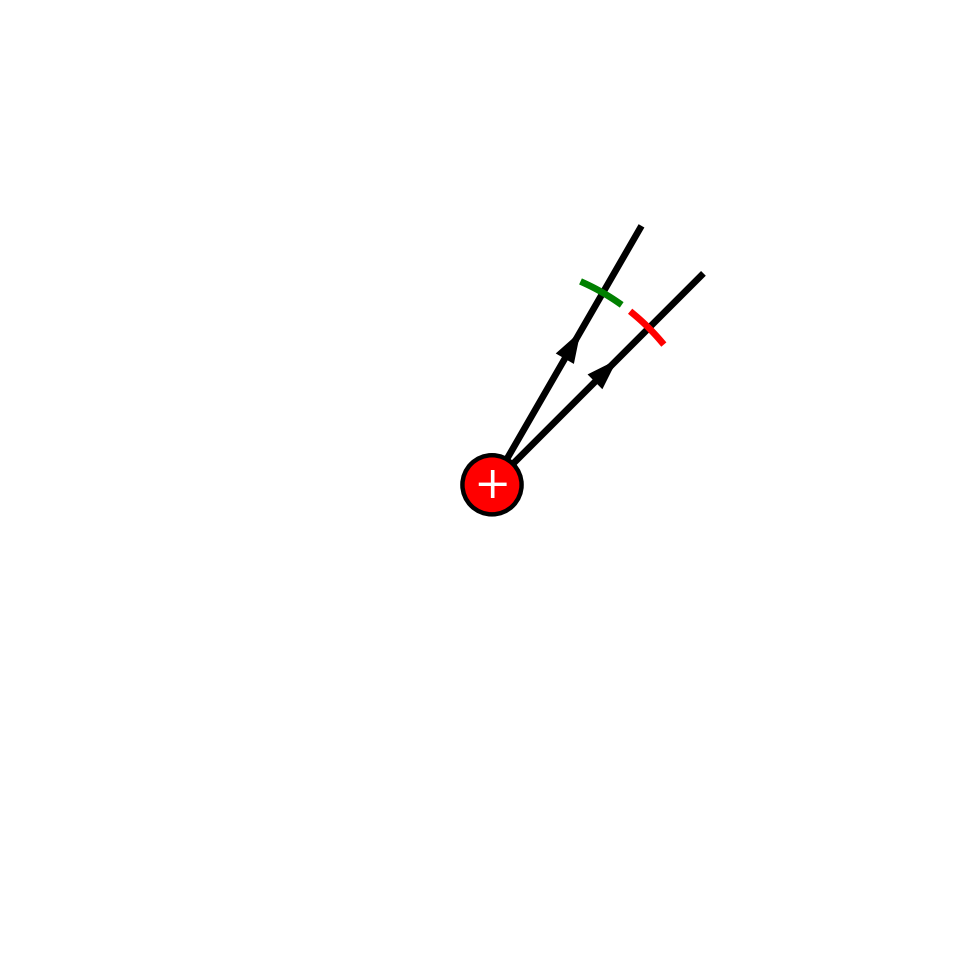
\includegraphics[width=0.75\columnwidth]{figs/seq/frame2}
\end{center}
\end{frame}
\begin{frame}
\frametitle{Coulomb potential}
\begin{center}
	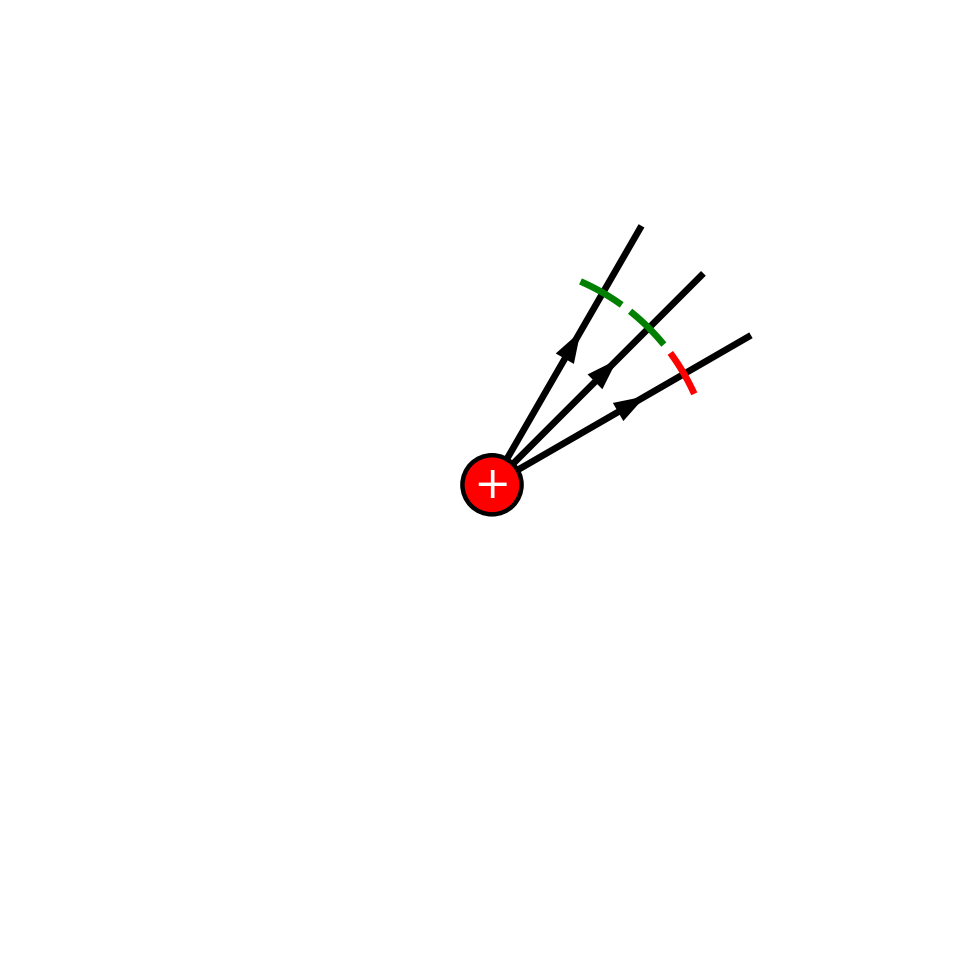
\includegraphics[width=0.75\columnwidth]{figs/seq/frame3}
\end{center}
\end{frame}
 \begin{frame}
\frametitle{Coulomb potential}
\begin{center}
	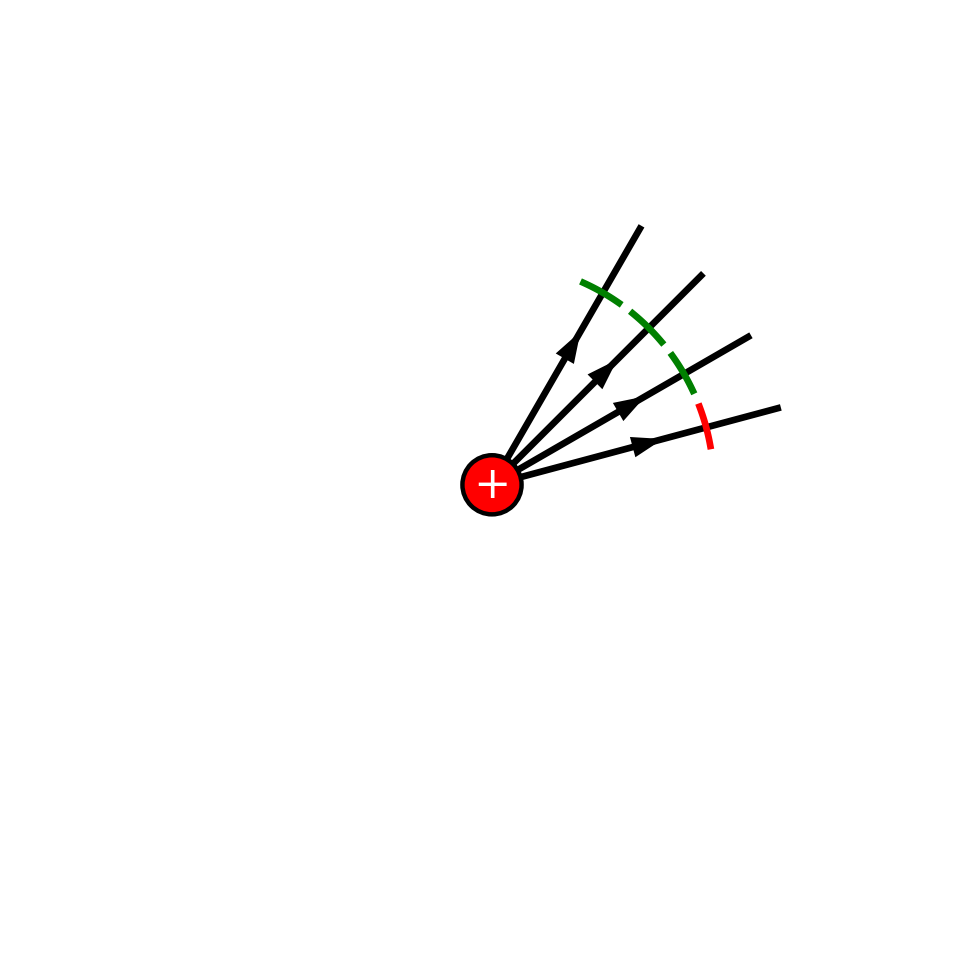
\includegraphics[width=0.75\columnwidth]{figs/seq/frame4}
\end{center}
\end{frame}
\begin{frame}
\frametitle{Coulomb potential}
\begin{center}
	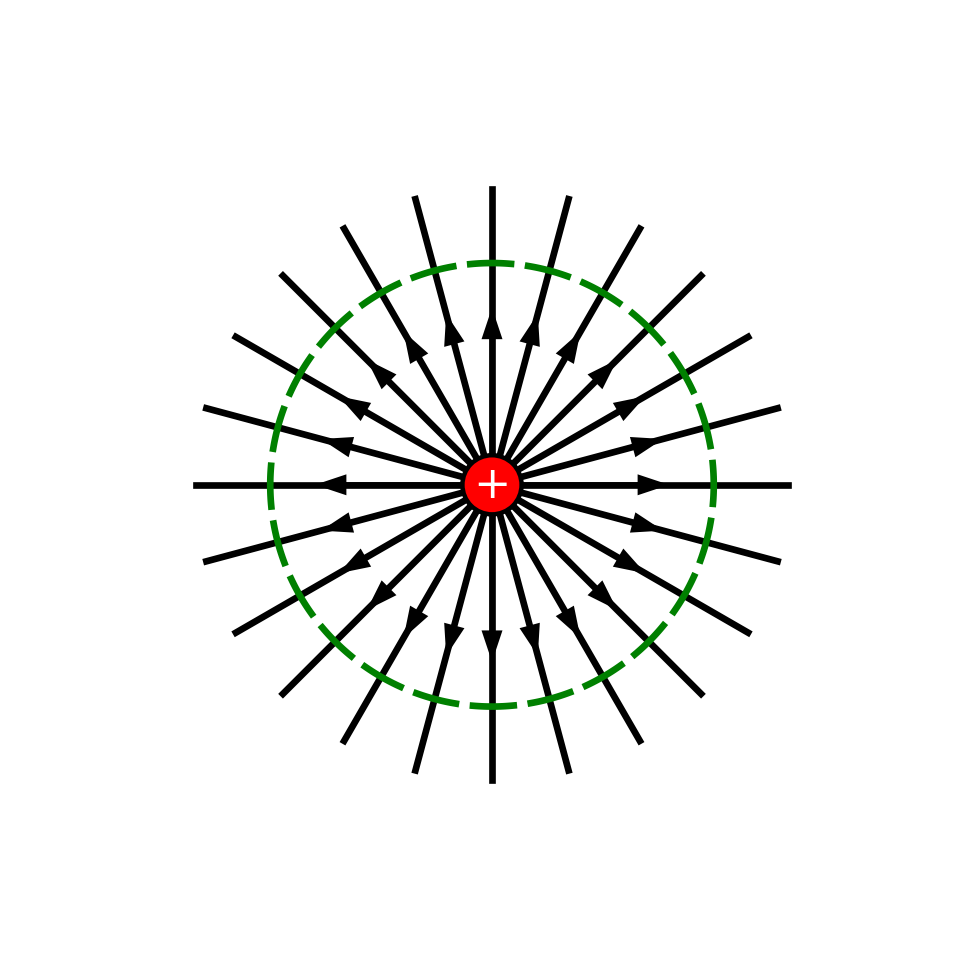
\includegraphics[width=0.75\columnwidth]{figs/seq/frame24}
\end{center}
\end{frame}




%%%%%%% end animation

\begin{frame}
\frametitle{Coulomb potential}
\small
\begin{center}

	\includegraphics[width=0.75\columnwidth]{figs/onecharge}
\end{center}

	
\end{frame}

\begin{frame}
	\frametitle{Multiple charges}
	
	For a system composed of multiple charges, the superposition principle holds for the potential as well:
	\begin{equation}
		V_{\rm total} =\sum_{k=1}^N V_k
	\end{equation}
	The potential is a scalar function that complements the picture provided by the field lines:\newline
	{\color{UniversityRed}\href{https://electric-charges.herokuapp.com/}{https://electric-charges.herokuapp.com/}}
	
	
\includegraphics[width=0.3\textwidth]{figs/qr-code}
	
	
	\end{frame}
	
%\begin{frame}
%\frametitle{Calculating $\vc{E}$ from V}
%\small 
%Let the potential $V(x,y,z) $ be a known function that only depends on $x$:
%$V(x) = 25 \unit{\volt}+12 \dfrac{\unit{\volt}}{\unit{\meter^2}} x^2$.  What is the corresponding electric field?\newline \pause
%
%We use $-\text{grad}V=\vc{E}$. Component-wise:
%$$\tiny E_x = -\dfrac{\partial V}{\partial x}= -24 x \dfrac{\unit{\volt}}{\unit{\meter^2}}, \quad E_y= -\dfrac{\partial V}{\partial y}=0,\quad E_z = -\dfrac{\partial V}{\partial z}=0$$
%So $\vc{E}= -24 x \dfrac{\unit{\volt}}{\unit{\meter^2}} \hi $, i.e. the field points towards regions of \hl{low potential}.
%
%
%\begin{center}
%	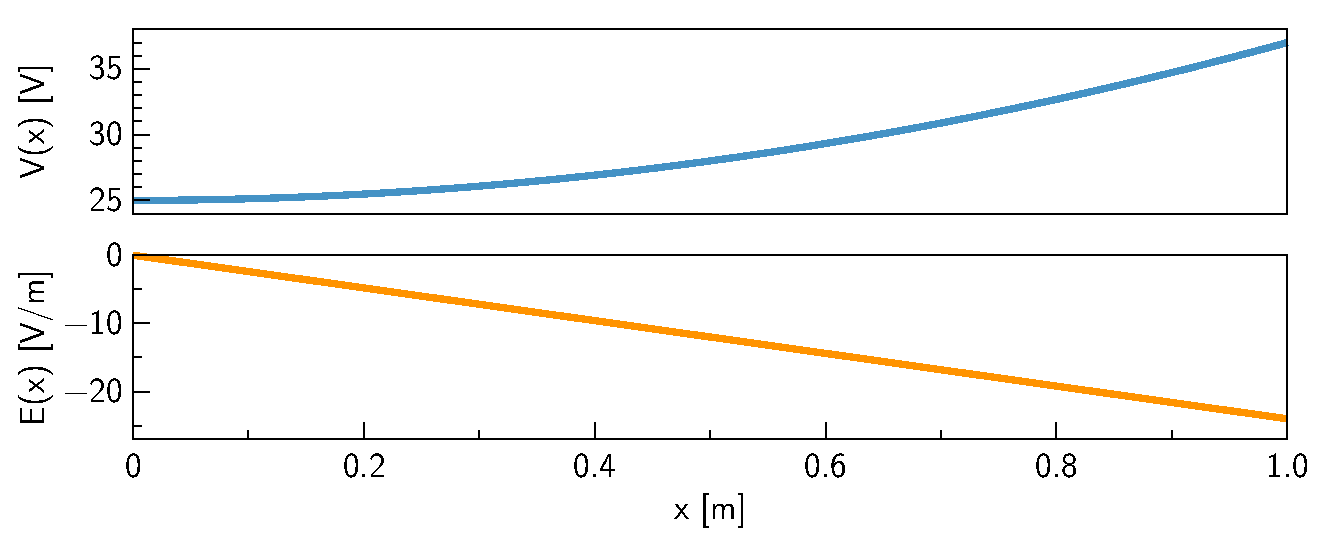
\includegraphics[width=0.7\textwidth]{figs/pot1d.pdf}
%\end{center}
%
%\end{frame}


\begin{frame}
\frametitle{Circulation}
\small

For a closed path $C$, path independence implies
\begin{block}{}
	\begin{equation}
	\mathcal{C} = \oint_C  \vc{E} \cdot d \vc{\ell} = 0
\end{equation}
\end{block}
For \textbf{any} closed path, the circulation of a conservative field is \textbf{zero}.\newline
\pause

Conservative forces/fields include:
\begin{itemize}
	\item the gravitational force and field	
	\item the electrostatic force and field
	\item the elastic force 
\end{itemize}

	
\hl{\textbf{Q:} Can you think of some \textbf{counter-examples}?}
\end{frame}

\begin{frame}
\frametitle{Lorentz force and magnetic field}
\small
The Lorentz force depends on both the magnetic field $\vc{B}$ and the velocity $\vc{v}$ of a charge $q$
\begin{equation}
	\vc{F}_m=q \vc{v} \times \vc{B},
\end{equation}
It is perpendicular to both $\vc{v}$ and $\vc{B}$ and the $\vc{v}$ dependence makes it \textbf{non-conservative}.\newline

%Important: the force is caused by the particle motion, not vice-versa.\newline

The work performed by $\vc{F}_m$  along any path is identically \textbf{zero}

\begin{equation}
	\int_i^f \vc{F}_m\cdot d\vc{\ell}=q\int_i^f  (\vc{v} \times \vc{B})\cdot d\vc{v}dt=0,
\end{equation}
(the scalar product of orthogonal vectors is zero).\newline
%
%\hl{The magnetic field does \textbf{no work} on the point charge}. We can formally define a potential $V_B$ such that $-\text{grad}V_B = \vc{B}$, but we cannot link it -in general- to a physical force.
\end{frame}

\begin{frame}
	\frametitle{Magnetic vs electric field}

	For the electric field, we can write the force on a point charge as $\vc{F}_e = q\vc{E}$.\newline
	
	For the magnetic field $\vc{B}$, the force is not simply proportional to the field, and there are \textbf{no magnetic charges}.\newline 
	
	The construction of the scalar potential $V$ from $\vc{E}$ \textbf{cannot be repeated }for $\vc{B}$.\newline
	
	\end{frame}


\begin{frame}
\frametitle{Magnetic vs electric field}

	In fact, the difference between $\vc{E}$ and $\vc{B}$ can be mathematically cast in terms of \textbf{circulation}
	\begin{align}
		\oint_C \vc{E}\cdot d \vc{\ell}&=0\\
		\oint_C \vc{B}\cdot d \vc{\ell}&=\mu_0 I_C\neq0\\
	\end{align}
	where $I_C$ is the current through the closed loop $C$. \newline 
	
	More on this in the next sessions.\newline
	
	
\end{frame}




\begin{frame}
\frametitle{Take-home messages}
\begin{enumerate}
	\item For conservative forces, the work done between two points in space is path-independent.
	\item The electrostatic field $\vc{E}$ is a \textbf{conservative vector field} with potential $V$:
	\begin{itemize}
	\item integral form $V_f-V_i=-\int_i^f \vc{E} \cdot d\vc{\ell}$
	\item local form $-\text{grad} V = \vc{E}$
	\end{itemize}
	\item There is no scalar potential for the magnetic field $\vc{B}$.
\end{enumerate}

\textbf{Remember:} this is valid for \textbf{static} fields.
\end{frame}

\end{document}